In this section the design of the trajectory followed by the spacecraft during the aerocapture and entry phase is presented. Also the motivation behind it, its sensitivity to changing atmospheric properties and the possibility to correct for these changes are explained. The main input with which the trajectory is calculated is the shape of the decelerator. This shape and the reasoning behind it is presented in Section \ref{subsec:infldes}. An overview of the aerocapture and entry phase trajectory is given in Figure \ref{fig:trajectory}.

\begin{figure}
	\centering
	
	\begin{subfigure}[b]{0.7\textwidth}
		\vspace{-22mm}
		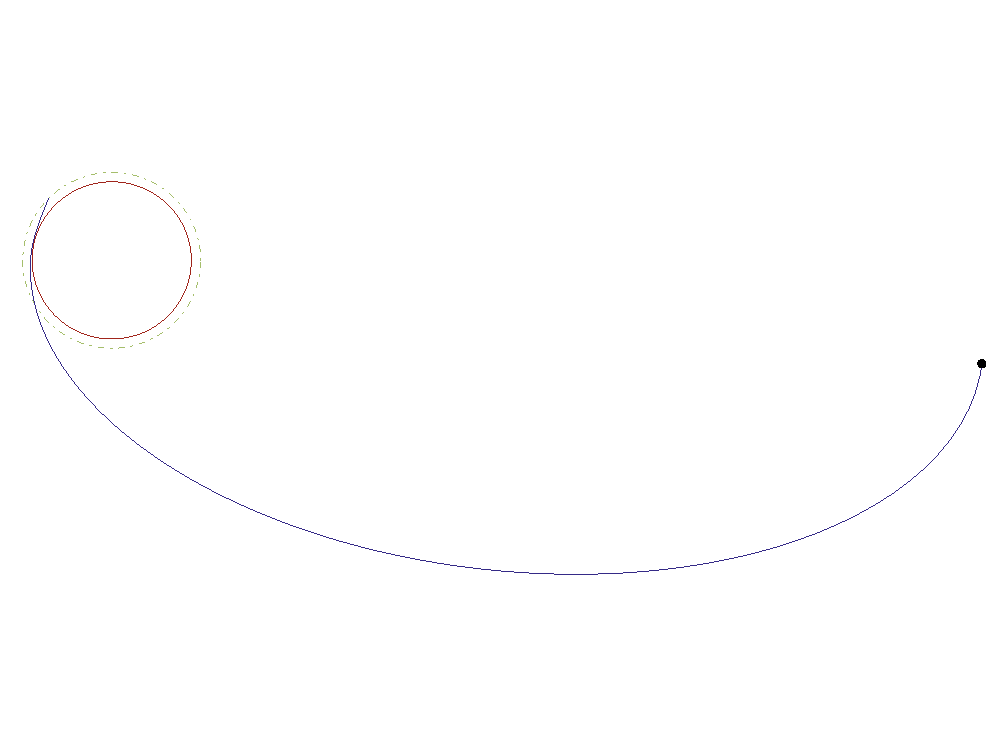
\includegraphics[width=\textwidth]{./Figure/Orbit/aerocapture_trajectory.pdf}
		\vspace{-25mm}
		\caption{The aerocapture trajectory visualised}
		\label{fig:capture_trajectory}
	\end{subfigure}
	\begin{subfigure}[b]{0.7\textwidth}
		\vspace{-10mm}
		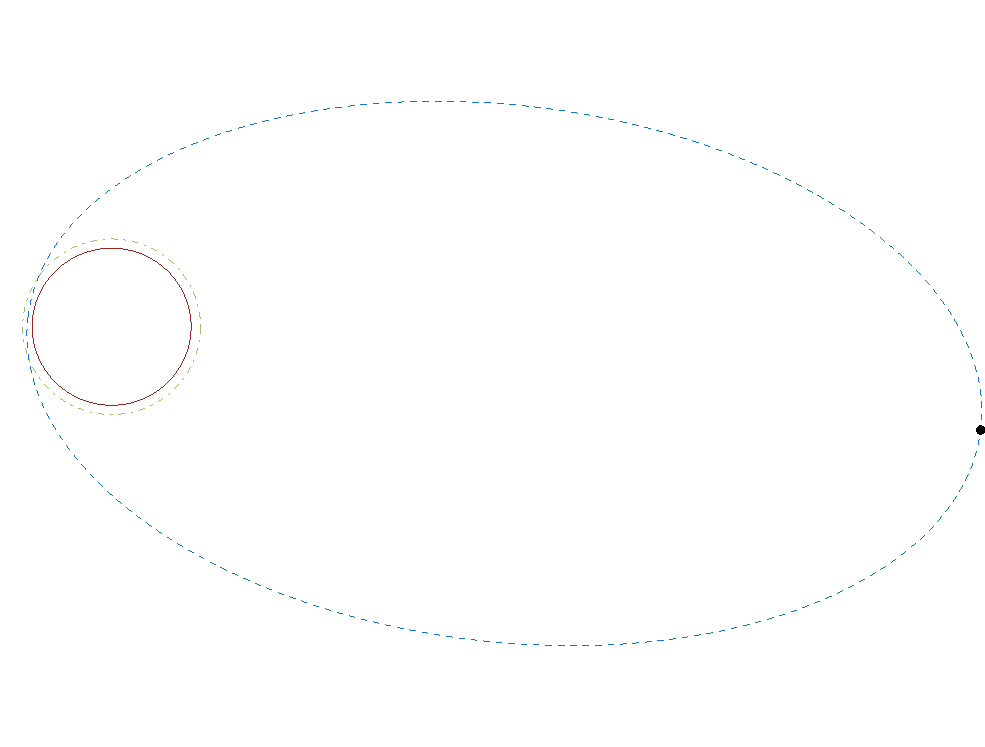
\includegraphics[width=\textwidth]{./Figure/Orbit/parking_trajectory.pdf}
		\vspace{-15mm}
		\caption{The parking orbit after the pericentre raise}
		\label{fig:parking_trajectory}
	\end{subfigure}
	\begin{subfigure}[b]{0.7\textwidth}
		\vspace{-22mm}
		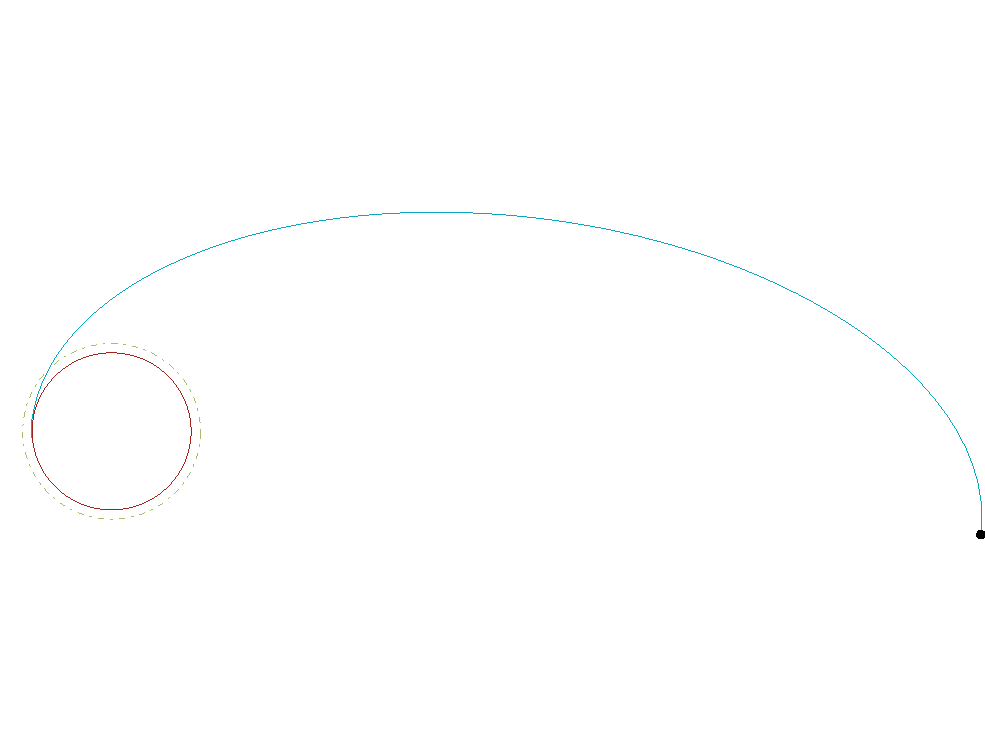
\includegraphics[width=\textwidth]{./Figure/Orbit/re-entry_trajectory.pdf}
		\vspace{-25mm}
		\caption{The re-entry trajectory after lowering the orbit}
		\label{fig:re_entry_trajectory}
	\end{subfigure}
	\caption[Visualisation of the spacecraft trajectory]{Visualisation of the spacecraft trajectory. The apocentre is shown with a black dot}
	\label{fig:trajectory}
\end{figure}

\subsubsection{Aerocapture} \label{sec:aerocapture}
The first phase of the trajectory is aerocapture, in which the objective is to lose enough energy to get in a Mars-synchronous orbit. The velocity that has to be obtained at the end of aerocapture in order to get in such an orbit is $4.53$ $\left[km \cdot s^{-1}\right]$. In Figure \ref{fig:orbit_aerocapture_data} it can be seen from the velocity profiles that they all end at this velocity.

Furthermore the trajectory was chosen as high through the atmosphere as possible to lower the required \gls{tps} and structural masses. A pass higher through the atmosphere decreases both the heat flux and peak dynamic pressure which are used to design the \gls{tps} and inflatable structure respectively.

These two objectives are conflicting since a higher altitude corresponds to a lower density, which makes it harder to achieve the required velocity change. In order to still reach the desired velocity, two options are available: with a longer aerocapture, the lower deceleration at higher altitudes is applied for enough time to reach the final velocity, and with a higher drag coefficient or frontal area the aerodynamic deceleration is increased for equal dynamic pressures.

A longer aerocapture can be achieved by improved control over the vehicle, which is accomplished by a higher lift coefficient. A longer aerocapture however, increases the total heat load, which may lead to a higher \gls{tps} mass.

In order to facilitate both objectives for aerocapture it is thus important that the aerodynamic shape has a high lift-to-drag ratio as well as a high drag coefficient. For the entry and descent phase conflicting objectives for the shape are found since a lower drag coefficient is required such that more time is available in this phase to manoeuvre. In Section \ref{sec:trajectory_summary} a conclusion is drawn on the properties needed from the design of the aerodynamic shape.

In Figure \ref{fig:orbit_aerocapture_data} the parameters that were recorded during the simulation are shown for the nominal trajectory and two trajectories created for a $10\%$ increase and decrease in atmospheric density. This change in density is based on the maximum estimated error in the \gls{esa} Mars climate database v5.2 \cite{Lewis2015}.

The bank control profile for the trajectories can be changed, by varying bank angle and timing, to attain the same exit velocity for each atmospheric density. This exit velocity is needed to get into a Mars-synchronous orbit. The fact that a bank control profile is available for each density proves that a density change of $\pm 10\%$ can be accounted for. However, some other parameters of the trajectory do change. The peak acceleration and dynamic pressure increase for a higher density. The \gls{tps} and inflatable structure should be sized on the worst case. Also the time passed and the position of exit (defined by $\tau$ in Figure \ref{fig:angles}) are different for each trajectory. These changes have a significant effect on the entry and descent phase. This effect will be explained in Section \ref{sec:entry_descent}.

\begin{sidewaysfigure}
	\centering
	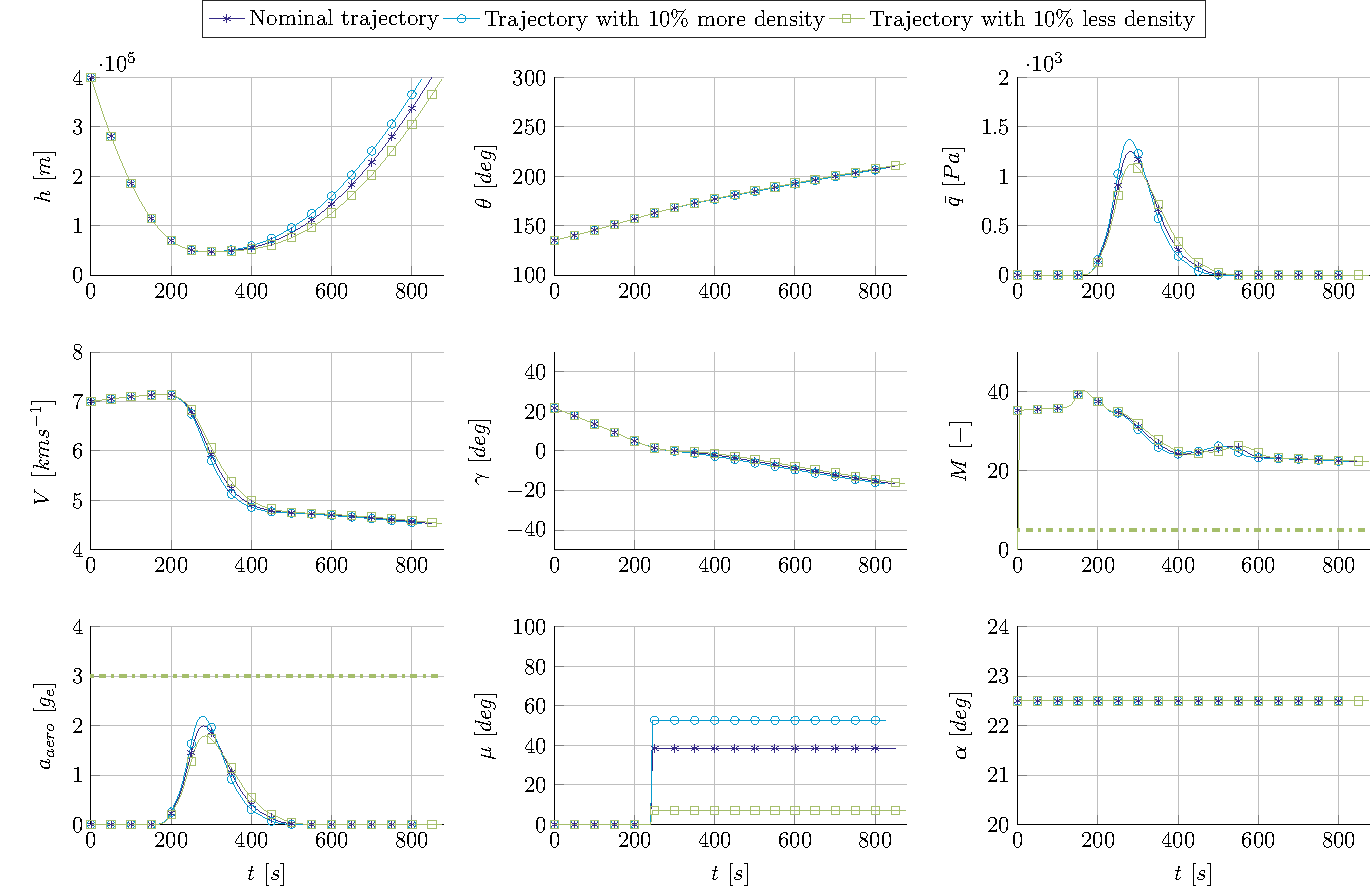
\includegraphics[width=0.99\textwidth]{Figure/Orbit/sensitivity_aerocapture.pdf}
	\caption[Results of the aerocapture trajectory for three different density profiles]{Results of the aerocapture trajectory for three different density profiles. The trajectories with modified density are corrected (changed \gls{sym:mu} profile) to maintain the same exit velocity. The horizontal dashed lines are design limits (for the \gls{sym:M} and \gls{sym:acc} plots) }
	\label{fig:orbit_aerocapture_data}
\end{sidewaysfigure}

\subsubsection{Parking orbit}\label{sec:parking_orbit}
After aerocapture the spacecraft goes into an elliptic orbit. In the apocentre a boost is given to raise the pericentre to $200 \left[km\right]$ above \gls{mola}. In this parking orbit the vehicle can wait for dust storms to vanish and can observe the entry conditions it will be subjected to. Because the parking orbit is Mars-synchronous the pericentre is over the same point on the Mars surface so entry conditions can be monitored for the actual entry point.

The first entry opportunity is after approximately one day from the start of the aerocapture and entry phase. From that moment every sol (Martian day) an opportunity for entry arises. This gives in total nine opportunities for entry in little over nine days. This is the maximum that can be achieved within the ten days that are available for the aerocapture and entry phase. In principle the spacecraft could stay in the parking orbit much longer if it would be necessary. However the current mission is fully designed for an aerocapture and entry phase of at most 10 days. i.e. crew operational items are insufficient to sustain a longer mission.

For every entry opportunity the decision to start entry has to be made half a sol before the entry. In the apocentre a boost opposite to the flight direction should be given to lower the pericentre.  When the vehicle reaches the atmosphere in this lower orbit the entry and descent phase begins.

\begin{figure}[h]
	\centering
	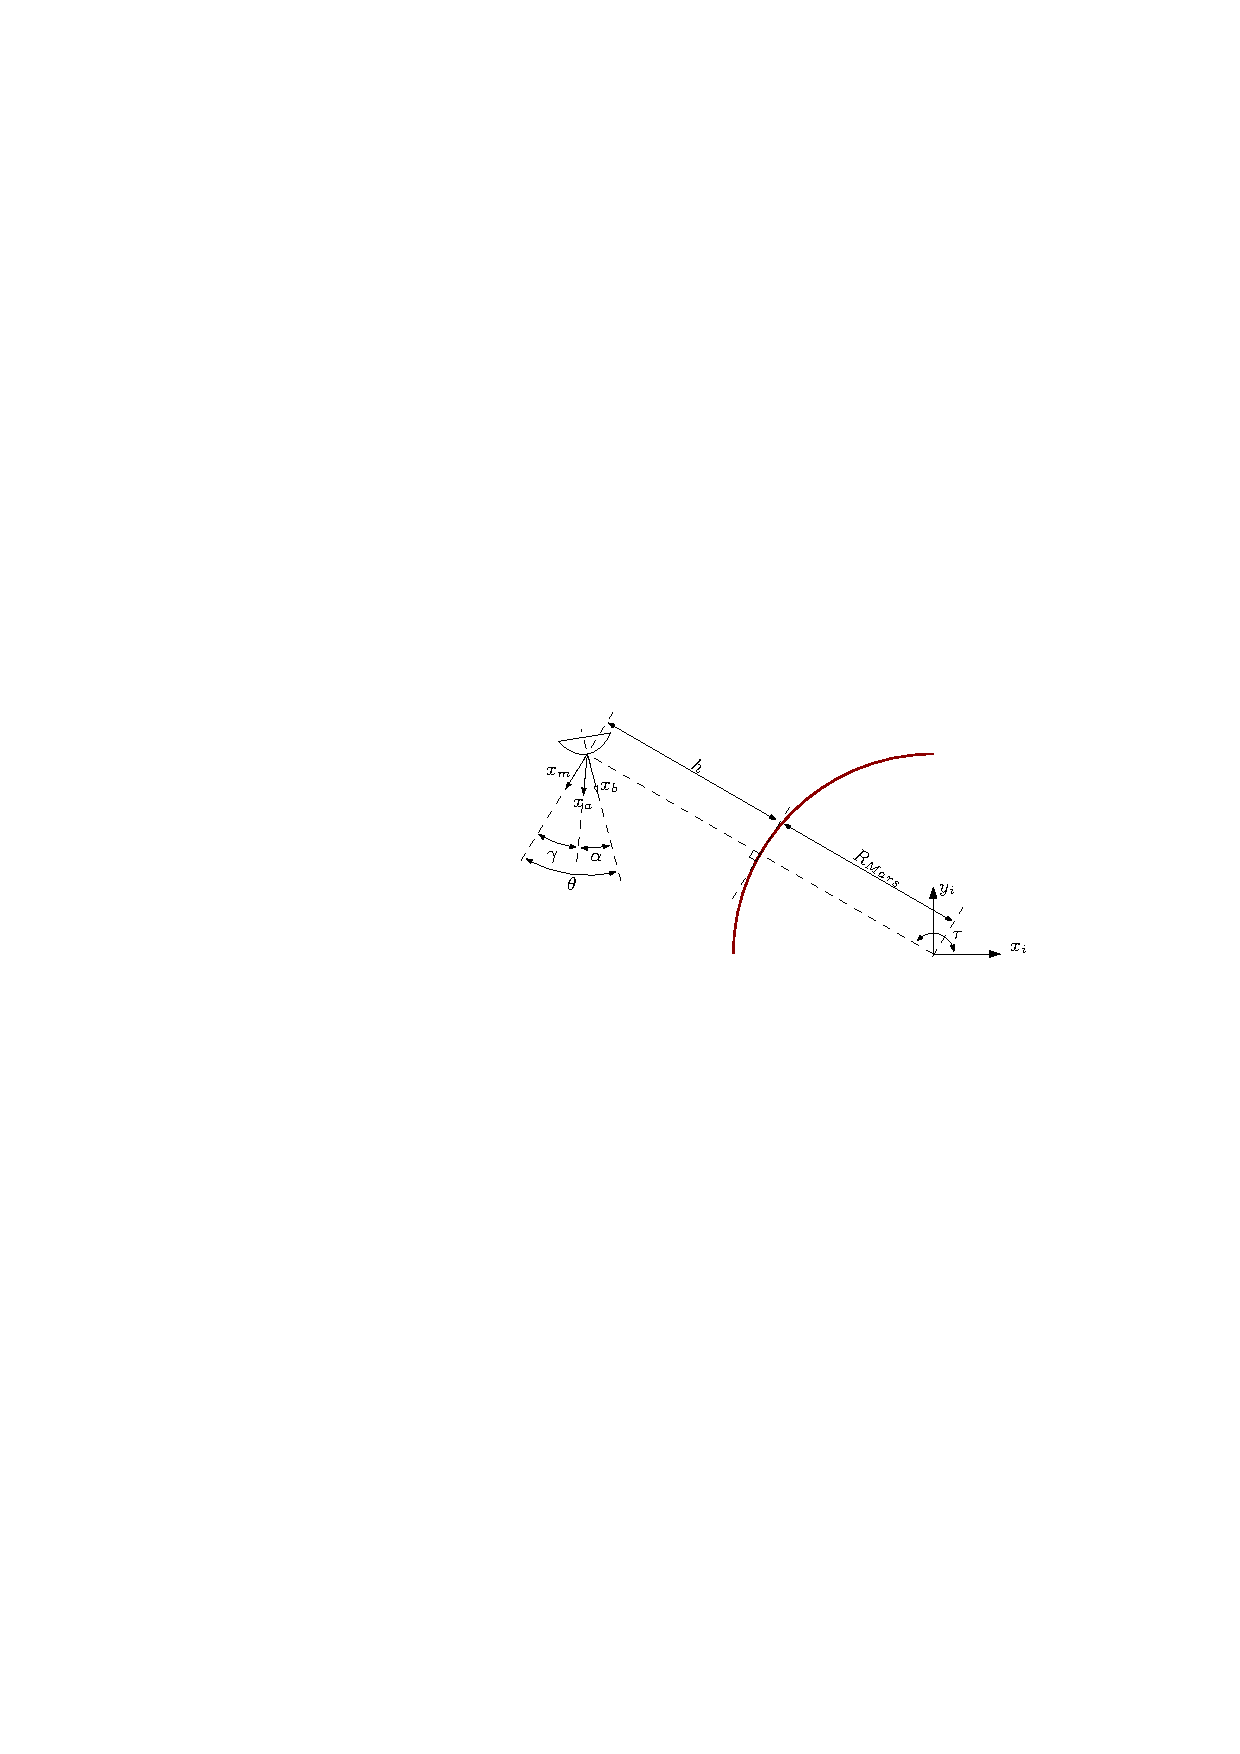
\includegraphics[width=0.7\textwidth]{Figure/Orbit/angles.pdf}
	\caption{The angles used in the simulation of the trajectory}
	\label{fig:angles}
\end{figure}

\subsubsection{Entry and descent}\label{sec:entry_descent}
The boost given in the apocentre before entry is determined such that the initial flight path angle ($\gamma$ as in Figure \ref{fig:angles}) of the entry is $17.2 \left[deg\right]$. Corresponding to this flight path angle an entry location (defined by $\tau$ in Figure \ref{fig:angles}) is dictated by the exit location of the aerocapture. With this location, flight path angle and the control as shown in Figure \ref{fig:orbit_entry_data}, the entry trajectory and final position are attained as shown in Figure \ref{fig:entry_mars}.

The objective of the entry and descent phase is to get to a height of $15 \left[km\right]$ with a velocity of $M = 5\left[-\right]$ while keeping the deceleration under 3\gls{con:ge}.

In order to keep the deceleration low, especially at the end of the descent, a low drag coefficient is required. This objective clearly conflicts with the properties needed for the aerocapture. As can be seen in Figure \ref{fig:orbit_entry_data} the deceleration at the end of the aerocapture and entry phase is right at the $3\gls{con:ge}$ limit for the nominal trajectory. Meaning the drag coefficient could not have gotten any higher.

In the last part of the descent also a high dynamic pressure is attained, which is the parameter that is the main input for inflatable structure design. The highest dynamic pressure is reached by the trajectory with a $10\%$ lower density.

In Figure \ref{fig:entry_mars} next to the nominal trajectory also two trajectories with a $10\%$ higher or lower density are plotted. The trajectory in the higher density atmosphere would land at a location before the nominal landing location if no change to the control is done. The trajectory that is shown for $10\%$ higher density is one with control that allows the vehicle to fly further (increased \gls{sym:mu}). This control causes the vehicle to overshoot the nominal landing location. Any point between these two margins is a possible landing location. It is thus proven that the nominal landing location can be achieved with $10\%$ higher density.

The trajectory for a $10\%$ lower density would normally overshoot the nominal landing location. The control is thus changed in order to push it towards the surface faster (lower \gls{sym:mu}). This control causes the vehicle to land before the nominal landing location. Again any point between these two margins is a possible landing location. This proves that the nominal landing location can be attained with $10\%$ lower density.

In Figure \ref{fig:entry_mars} it can also be seen that the entry locations for each trajectory is different. This flows down from the aerocapture where the exit location for these trajectories where different as well.

The time passed during both the aerocapture and the entry and descent phases are also different for each trajectory. During this time the landing location has rotated with Mars in the same direction as the flight direction of the vehicle. Three points for the nominal landing location can be distinguished in Figure \ref{fig:entry_mars}. Each point for the time one of the trajectories would arrive.

\begin{figure}[h]
	\centering
	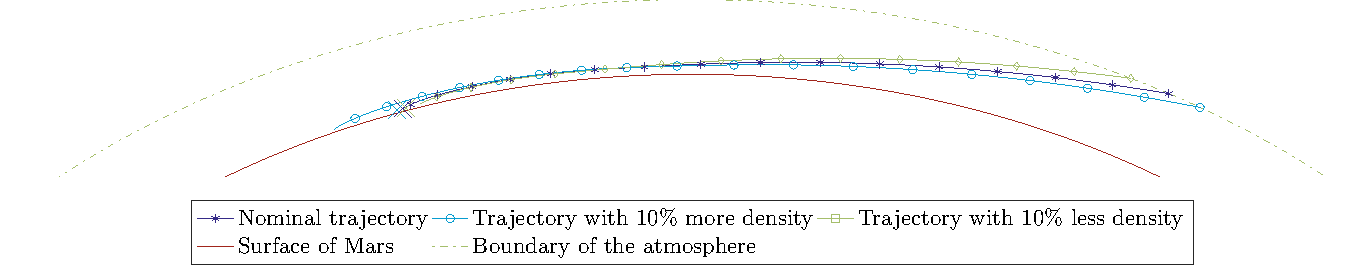
\includegraphics[width=0.99\textwidth]{Figure/Orbit/entry_mars.pdf}
	\caption[The re-entry trajectory for three different density profiles]{The re-entry trajectory for three different density profiles. The trajectories with modified density are corrected (changed \gls{sym:mu} profile) to show the ability to reach the desired landing location.}
	\label{fig:entry_mars}
\end{figure}

In Figure \ref{fig:orbit_entry_data} it can be seen that the Mach number at a height of $15 \left[km\right]$ is approximately $5$ for all trajectories. The entry trajectory with a lower density is the shortest, however it also decelerates fastest overshooting the $3\gls{con:ge}$ requirement by $23\%$. This higher deceleration is needed to reach the required velocity of $M=5 \left[-\right]$.

The entry trajectory with a higher density is the longest. The deceleration is also faster than for the nominal trajectory and it also overshoots the $3\gls{con:ge}$ requirement by $11\%$. This higher deceleration is caused by the denser atmosphere at a height of $15 \left[km\right]$.

\begin{sidewaysfigure}
	\centering
	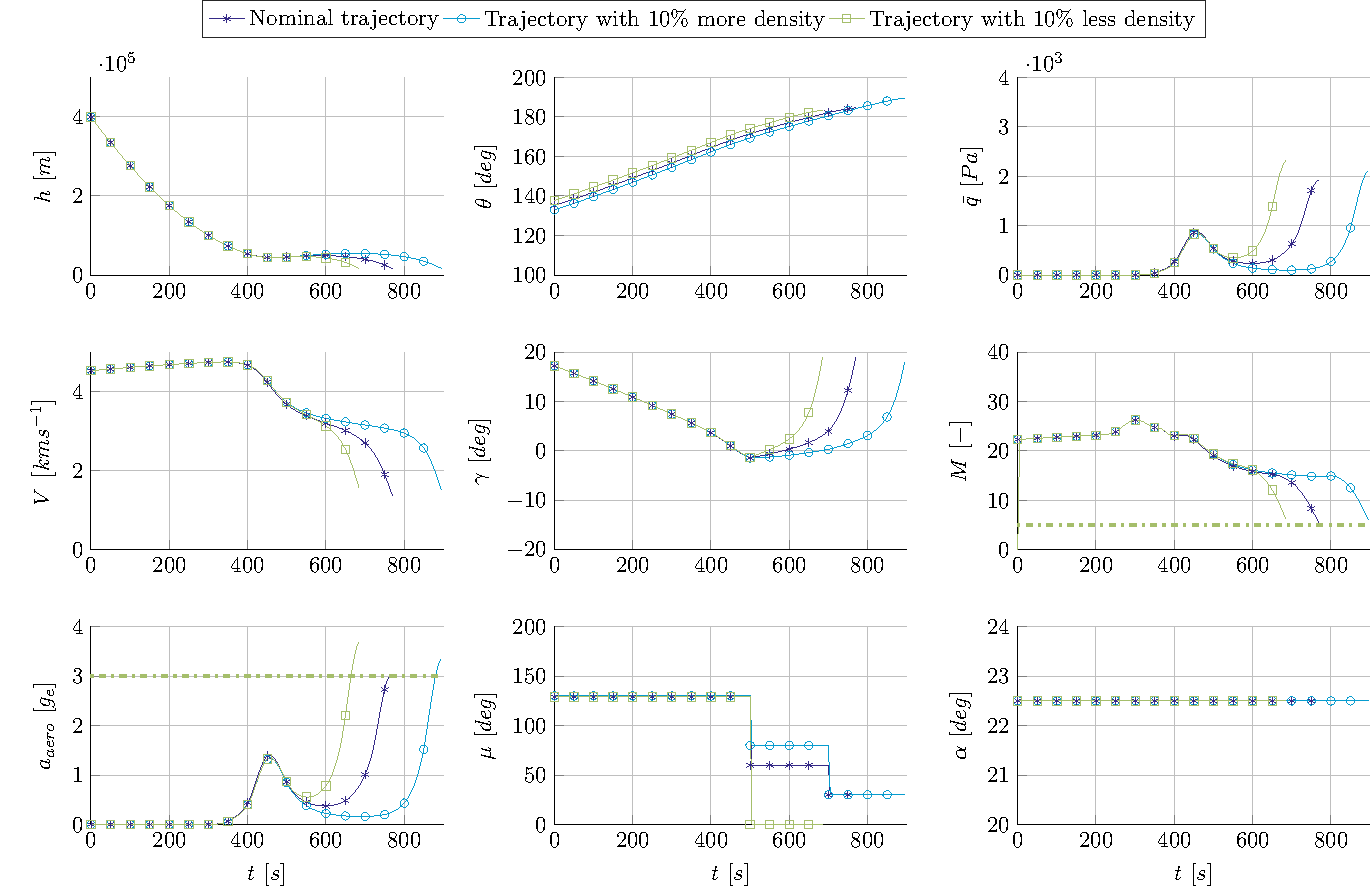
\includegraphics[width=0.99\textwidth]{Figure/Orbit/sensitivity_entry.pdf}
	\caption[Results of the re-entry trajectory for three different density profiles]{Results of the re-entry trajectory for three different density profiles. The trajectories with modified density are corrected (changed \gls{sym:mu} profile) to show the ability to reach the desired landing location. The horizontal dashed lines are design limits (for the \gls{sym:M} and \gls{sym:acc} plots)}
	\label{fig:orbit_entry_data}
\end{sidewaysfigure}

\subsubsection{Required properties for aerodynamic shape design} \label{sec:trajectory_summary}
The required aerodynamic properties for the different parts of the aerocapture and entry phase are conflicting. For the aerocapture phase a high drag coefficient as well as a high lift coefficient is needed. For the entry phase still a high lift coefficient is needed, however also a low drag coefficient is required.

Compromising between these requirements an angle of attack has been chosen at which the $\gls{sym:L}\cdot\gls{sym:D}^{-1}$ is maximal in order to maximise the lift for certain drag. The aerodynamic shape should be designed in such a way that the drag at maximum $\gls{sym:L}\cdot\gls{sym:D}^{-1}$ is a perfect compromise between the objectives for the aerocapture and entry \& descent phases.
